  \documentclass[12pt]{exam}
\usepackage{amsthm}
\usepackage{libertine}
\usepackage[utf8]{inputenc}
\usepackage[margin=1in]{geometry}
\usepackage{amsmath,amssymb}
\usepackage{multicol}
\usepackage[shortlabels]{enumitem}
\usepackage{siunitx}
\usepackage{float}
\usepackage{cancel}
\usepackage{graphicx}
\usepackage[T1]{fontenc}
\usepackage[spanish]{babel}
\usepackage{pgfplots}
\usepackage{listings}
\usepackage{tikz}
\usepackage{xcolor}
\usepackage{xparse}


\pgfplotsset{width=10cm,compat=1.9}
\usepgfplotslibrary{external}
\tikzexternalize

\NewDocumentCommand{\codeword}{v}{%
\texttt{\textcolor{blue}{#1}}%
}

\newcommand{\class}{Diseño y Análisis de Algoritmos} % This is the name of the course 
\newcommand{\examnum}{Proyecto 2} % This is the name of the assignment
\newcommand{\examdate}{\today} % This is the due date
\newcommand{\timelimit}{}





\begin{document}
\pagestyle{plain}
\thispagestyle{empty}

\noindent
\begin{tabular*}{\textwidth}{l @{\extracolsep{\fill}} r @{\extracolsep{6pt}} l}
	\textbf{\class} & \textbf{Nombre:} & \textit{Sergio Montoya}\\ %Your name here instead, obviously 
	\textbf{\examnum} &&\\
	\textbf{\examdate} &&
\end{tabular*}\\
\rule[2ex]{\textwidth}{2pt}
% ---

\section{Explicación del Algoritmo}

Para iniciar, debemos definir un grafo. Este grafo estará representado por una matriz de adyacencia. Cada uno de los vértices sera una célula y sera representado sin colación por su identificador (En concreto en la matriz de adyacencia es su identificador $-1$). Ademas, existe un arco entre dos vértices si comparten peptidos y si la distancia entre ambos es menor a la distancia máxima en la que puede ocurrir una conexión. Ademas, cada arco tiene un peso correspondiente al numero de peptidos que comparten. Esto nos da un grafo no dirigido  con pesos.

Lo que nos interesa es saber el numero máximo de mensajes que se pueden enviar por este grafo, esto esencialmente es un problema de flujo. Lo que nos interesa ver es cual de las células Calculadoras tiene un mayor efecto en el flujo total.

Para esto se hizo uso del algoritmo de Ford-Fulkerson. Este algoritmo es ejecutado sobre el grafo original y luego se aplica de manera subsecuente a el grafo en donde fue retirada la célula calculadora concreta.

En un principio dudaba de aplicar Ford-Fulkerson en cada paso. Sin embargo, es necesario hacerlo pues es posible que la ruta de flujo cambie radicalmente y que el flujo que pasa por la neurona que estamos mirando pueda ser tomado por otra en su mayoría afectando mínimamente el flujo máximo total.

\begin{figure}[H]
  \centering
  \includegraphics[width=0.8\textwidth]{img/explicacion.png}
  \caption{Ejemplo del algoritmo probando para una de las células calculadoras.}
  \label{fig:explicacion}
\end{figure}

\section{Complejidad}

Para la complejidad temporal la tomaremos solamente de la solución como tal. La construcción del grafo apartar de la entrada tiene una complejidad polinomial pero podría variar ampliamente. En concreto, trabajaremos con la función \codeword{get_max_flow} que esta aproximadamente en la linea 210.

\subsection{Temporal}

Lo primero que hace esta función es crear una nueva copia. Esto tiene una complejidad $O\left( V^2 \right) $. Luego de esto remueve la célula que se le indica lo cual es una complejidad de $O\left( V \right)$ y por ultimo calcula el flujo maximo con FORD-FULKERSON lo cual tiene una complejidad de $O\left( \left| V \right| \cdot E^2 \right) $. Por lo tanto esta función tiene una complejidad de \[
O\left( V^2 \right) + O\left( V \right) + O\left( \left| V \right| \cdot E^2 \right) = O\left( \left| V \right| \cdot E^2 \right) 
.\] Ahora bien, esta función es ejecutada $C$ veces donde $C$ es el numero de células Calculadoras. En el peor de los casos $C = V$ por lo tanto para el peor de los casos la complejidad temporal es: \[
O\left( V \cdot \left| V \right| \cdot E^2 \right) 
.\] 

\subsection{Espacial}

Para la complejidad espacial debemos tomar encuenta que esta función crea una copia de la matriz lo que tiene un costo de $O\left( V^2 \right) $ y ademas FORD-FULKERSON tiene un costo de $O\left( V \right) $. Por lo tanto la complejidad total seria \[
O\left( V^2 \right) + O\left( V \right)  = O\left( V^2 \right) 
.\] 

\section{Preguntas Comprensión}

\subsection{Primera Pregunta}

En ese caso, se sabe que el numero mínimo de mensaje que podría tener el flujo es el de la suma de los mensajes que pasan de las células iniciadoras a las células ejecutoras. Pues incluso si se apagaran todas las células calculadoras seguirían estando estos caminos.

\subsection{Segunda Pregunta}

En ese caso el numero de mensajes máximo seria el del numero de células calculadoras pues serian como un cuello de botella que solo permitiría que el flujo máximo fuera de a uno en ellas.

\end{document}
